% Copyright (c) 2016-2020 The ALF project.
% This is a part of the ALF project documentation.
% The ALF project documentation by the ALF contributors is licensed
% under a Creative Commons Attribution-ShareAlike 4.0 International License.
% For the licensing details of the documentation see license.CCBYSA.

% !TEX root = doc.tex

%------------------------------------------------------------
\subsubsection{Langevin dynamics} \label{sec:langevin}
%------------------------------------------------------------

For models that include continuous real fields $\vec{s} \equiv \left\{s_{k,\tau} \right\}$ there is the option of using Langevin dynamics for the updating scheme, by setting  the variable \texttt{Langevin} to \texttt{.true.}. This corresponds to a  stochastic differential equation for the fields. They acquire a discrete Langevin time $\tl$ with step width $\delta \tl$ and satisfy the stochastic differential equation
\begin{equation}\label{eqn:langevin}
   \ve{s}(\tl +  \delta \tl)    =    \ve{s}(\tl)    - Q \frac{\partial S( \ve{s}(\tl)) }{\partial    \ve{s}(\tl) }    \delta \tl     +\sqrt{2 \delta \tl Q} \ve{\eta}(\tl).
\end{equation}
Here, $ \ve{\eta}(\tl) $ are independent Gaussian stochastic variables satisfying:
\begin{equation}
        \langle  \eta_{k,\tau}(\tl) \rangle_{\eta}  = 0   \quad\text{and}\quad    \langle  \eta_{k,\tau}(\tl)  \eta_{k',\tau'}(\tl') \rangle_{\eta}  = \delta_{k,k'} \delta_{\tau,\tau'} \delta_{\tl,\tl'},
\end{equation}
$S( \ve{s}(\tl))$ is an arbitrary real action and $Q$ is an arbitrary positive definite matrix. By default $Q$ is equal to the identity matrix, but a proper choice can help accelerate the update scheme, as we discuss below. 
We refer the reader to  Ref.~\cite{Gardiner}  for an in-depth introduction to stochastic differential equations.
To see that the above  indeed produces the desired probability distribution in the long Langevin time limit, we can transform the Langevin equation into the corresponding Fokker-Plank one.  Let
$P(\ve{s}, \tl) $ be the distribution of fields at Langevin time $\tl$. Then,
\begin{equation}
        P(\ve{s}, \tl  + \delta \tl )    = \int D\ve{s}'  P  (\ve{s}', \tl  )    \left\langle    \delta \left(  \ve{s} - \left[ \ve{s}'   - Q\frac{\partial S(\ve{s}' )}{\partial    \ve{s}' }   \delta \tl     +\sqrt{2 \delta \tl Q} \vec{\eta}(\tl)  \right]    \right) \right\rangle_{\eta},
\end{equation}
where $\delta$ corresponds to the $L_\mathrm{trotter} M_I $ dimensional Dirac $\delta$-function.   Taylor expanding  up to order $\delta \tl$  and averaging over the stochastic variable yields:
\begin{multline}
P(\ve{s}, \tl  + \delta \tl ) = \int D\ve{s'}  P  (\ve{s}', \tl  )   \left(   \delta \left(  \ve{s}' - \ve{s}   \right)
-   \frac{\partial  }{\partial    \ve{s'} } \delta \left(  \ve{s}' - \ve{s} \right) Q \frac{\partial S(\ve{s'}) }{\partial    \ve{s'} }  \delta \tl   \right.  \\
   \left. + \frac{\partial  }{\partial    \ve{s'} } Q  \frac{\partial  }{\partial    \ve{s}' }  \delta \left(  \ve{s}' - \ve{s}\right)    \delta \tl
\right)  + {\cal O}  \left(  \delta \tl^2 \right).
\end{multline}
Partial integration  and taking the limit of infinitesimal time steps   gives the Fokker-Plank equation
\begin{equation}
         \frac{\partial  }{\partial   \tl}  P( \ve{s}, \tl)  =  \frac{\partial  }{\partial    \ve{s} }  \left( P( \ve{s}, \tl)  Q\frac{\partial S(\ve{s}) }{\partial     \ve{s} }   +
        Q  \frac{\partial P(\ve{s},\tl) }{\partial     \ve{s} }
         \right) .
\end{equation}
The stationary,  $ \frac{\partial  }{\partial   \tl}  P( \ve{s}, \tl) =0$,  normalizable,  solution to the above equation corresponds to the desired probability distribution:
\begin{equation}\label{eqn:langevin_solution}
          P(\ve{s}) =  \frac{ e^{ - S(\ve{s}) } }   {   \int D \ve{s}  e^{ - S(\ve{s}) } }.
\end{equation}
Taking into account a potential negative sign problem, the action   for our general model reads:
\begin{equation}
	\overline{S}(C)   = -  \ln \left|  \text{Re} \left\{  e^{-S(C)} \right\} \right| 
\end{equation}
where  $S(C) $  is defined in Eq.~\eqref{eqn:partition_2}. Hence, 
\begin{equation}
   \frac{ \partial{\overline{S}(C)}} {\partial s_{k,\tau} }    =   \frac{1}{\text{Re} \left\{e^{i \phi(C)}\right\} } \text{Re} \left\{  e^{i\phi(C)}\frac{ \partial S (C)} {\partial s_{k,\tau} }   \right\}
\end{equation}
with
\begin{equation}
	e^{i \phi(C)}  =   \frac{e^{- S(C)}}{| e^{-S(C)}  |}
\end{equation}
corresponding to the variable \texttt{PHASE}  in the ALF-package. 

Therefore, to  formulate  the Langevin dynamics  we need  to estimate the forces:
\begin{equation}
	\frac { \partial S (C)}{\partial s_{k,\tau} } =\frac { \partial S_{0}(C)}{\partial s_{k,\tau} } +  \frac { \partial S^F(C)}{\partial s_{k,\tau} },
\end{equation}
with the fermionic part of the action being
\begin{multline}
S^F(C) =   - \ln \left\{  \left( \prod_{k=1}^{M_V} \prod_{\tau=1}^{L_{\mathrm{Trotter}}} \gamma_{k,\tau} \right)
    e^{ N_{\mathrm{col}}\sum\limits_{s=1}^{N_{\mathrm{fl}}} \sum\limits_{k=1}^{M_V} \sum\limits_{\tau = 1}^{L_{\mathrm{Trotter}}}\sqrt{-\Delta \tau U_k}  \alpha_{k,s} \eta_{k,\tau} } 
  \right.  \\
    \left. \times
	\prod_{s=1}^{N_{\mathrm{fl}}}\left[\det\left(  \mathds{1} + 
	\prod_{\tau=1}^{L_{\mathrm{Trotter}}}   
	\prod_{k=1}^{M_V}   e^{  \sqrt{ -\Delta \tau  U_k} \eta_{k,\tau} {\bm V}^{(ks)} }   \prod_{k=1}^{M_I}   e^{  -\Delta \tau s_{k,\tau}  {\bm I}^{(ks)}}  
	\prod_{k=1}^{M_T}   e^{-\Delta \tau {\bm T}^{(ks)}} 
	\right) \right]^{N_{\mathrm{col}}} \right\}  .
\end{multline}
The forces must be bounded for Langevin dynamics to work well. If this condition is violated the results produced by the code are \emph{not reliable}. 

One possible source of divergence is the determinant in the fermionic action. Zeros lead to unbounded forces and, in order to mitigate this problem, we adopt a variable time step.  The user provides an upper bound to the fermion force, \texttt{Max\_Force} and, if the maximal force in a configuration, \texttt{Max\_Force\_Conf}, is larger than \texttt{Max\_Force}, then the time step is rescaled as 
\begin{equation}
     \tilde{\delta \tl}   =  \frac{ \texttt{Max\_Force}} {\texttt{Max\_Force\_Conf}} \; \texttt{*} \; \delta \tl.
\end{equation}
With the adaptive time  step,  averages are computed as: 
\begin{equation} \label{eq:obs_varstep}
   \langle \hat{O} \rangle = \frac{ \sum_n (  \tilde{\delta \tl}  )_n  \sgn(C_n)   \frac{e^{-S(C_n)}}{\Re \left[e^{-S(C_n)} \right]}   \langle \langle \hat{O} \rangle   \rangle_{(C_n)} } {\sum_n (  \tilde{\delta \tl}  )_n  \sgn(C_n)  }. 
\end{equation}
where  $\sgn(C_n)$   is defined in Eq.~\eqref{Sign.eq}.    In this context the adaptive time step corresponds to the variable \texttt{Mc\_step\_weight}  required for the measurement routines (see Sec.~\ref{sec:obs}).  {\color{red}{FFA. We will have to update this section}}

A possible way to reduce autocorrelation times is to employ Fourier acceleration \cite{Batrouni85,Batrouni19}. As we see from Eq.~\eqref{eqn:langevin_solution}, the choice of the matrix $Q$ does not alter the probability distribution obtained from the Langevin equation. The main idea of Fourier acceleration is to exploit this freedom and use $Q$ to scale the Langevin time step $\delta t_l$ depending on the momentum of the fields $\vec{s}$. Namely, so that the field components with low momenta are multiplied by an effective larger step size compared to components with high momenta \cite{Davies86}. The modified Langevin equation reads:
\begin{equation}
   \ve{s}(\tl +  \delta \tl)    =    \ve{s}(\tl)    - \hat{F}^{-1} \left[ Q \hat{F}\left[\frac{\partial S( \ve{s}(\tl)) }{\partial    \ve{s}(\tl) } \right]   \delta \tl     +\sqrt{2 \delta \tl Q} \hat{F}\left[\ve{\eta}(\tl)\right] \right],
\end{equation}
with $\hat{F}$ being a Fourier transformation to momentum space. Currently an implementation of Fourier acceleration is not available in ALF, but can be included by the user.

In order to use Langevin dynamics the user also has to provide the Langevin time step \texttt{Delta\_t\_Langevin\_HMC},  the maximal force \texttt{Max\_Force},  set  \texttt{Global\_update\_scheme = Langevin} in the \texttt{parameter} file.  Furthermore, the   forces   $ \frac{ \partial S_{0}(C)}{\partial s_{k,\tau}}  $  are to be specified in the routine \texttt{Ham\_Langevin\_HMC\_S0}  of the Hamiltonian files.  The Langevin update   for a general Hamiltonian  is carried out in the module  \texttt{Langevin\_HMC\_mod.F90}.   In particular the  fermion forces, 
\begin{equation}
 \frac { \partial S^F(C)}{\partial s_{k,\tau} } 
 	=  \Delta \tau {N_{\mathrm{col}}} \sum\limits_{s=1}^{N_{\mathrm{fl}}} \Tr{\left[ \bm{I}^{(ks)} \left(\mathds{1} - \bm{G}^{(s)}(k,\tau) \right) \right]},
\end{equation}
are computed in this module. 
In the above, we  introduce a Green function that depends on the time slice $\tau$  and the interaction term $k$ to which the corresponding field $s_{k,\tau}$ belongs:
\begin{equation}\label{eqn:green_langevin}
G_{x,y}^{(s)}(k,\tau) = \frac{\Tr{\left[ \hat{U}_{(s)}^{<}(k,\tau) \hat{c}_{x,s}^{\phantom\dagger} \hat{c}_{y,s}^{\dagger} \hat{U}_{(s)}^{>}(k,\tau) \right]} }
{\Tr{\left[ \hat{U}_{(s)}^{<}(k,\tau)\hat{U}_{(s)}^{>}(k,\tau) \right]}},
\end{equation}
where the following definitions are used
\begin{align}
 \hat{U}_{(s)}^{<}(k',\tau') &= \prod_{\tau=\tau'+1}^{L_{\text{Trotter}}}  \left( \hat{U}_{(s)}(\tau) \right)
  \prod_{k=1}^{M_V} e^{\sqrt{-\Delta\tau U_k}  \eta_{k,\tau'} \hat{\vec{c}}_{s}^{\dagger} \bm{V}^{(ks)} \hat{\vec{c}}_{s}^{\phantom\dagger}}
\prod_{k=k'+1}^{M_I} e^{-\Delta\tau s_{k,\tau'} \hat{\vec{c}}_{s}^{\dagger} \bm{I}^{(ks)} \hat{\vec{c}}_{s}^{\phantom\dagger}}, \\
 \hat{U}_{(s)}^{>}(k',\tau') &= \prod_{k=1}^{k'} e^{-\Delta \tau s_{k,\tau'}  \hat{\vec{c}}_{s}^{\dagger} \bm{I}^{(ks)} \hat{\vec{c}}_{s}^{\phantom\dagger}}
  \prod_{k=1}^{M_T}   e^{-\Delta\tau  \hat{\vec{c}}_{s}^{\dagger} \bm{T}^{(ks)} \hat{\vec{c}}_{s}^{\phantom\dagger}} 
  \prod_{\tau=1}^{\tau'-1}  \left( \hat{U}_{(s)}(\tau) \right), \\
  \hat{U}_{(s)}(\tau) &= \prod_{k=1}^{M_V} e^{\sqrt{-\Delta\tau U_k}  \eta_{k,\tau} \hat{\vec{c}}_{s}^{\dagger} \bm{V}^{(ks)} \hat{\vec{c}}_{s}^{\phantom\dagger}} 
  \prod_{k=1}^{M_I} e^{-\Delta\tau s_{k,\tau} \hat{\vec{c}}_{s}^{\dagger} \bm{I}^{(ks)} \hat{\vec{c}}_{s}^{\phantom\dagger}}
    \prod_{k=1}^{M_T}   e^{-\Delta\tau  \hat{\vec{c}}_{s}^{\dagger} \bm{T}^{(ks)} \hat{\vec{c}}_{s}^{\phantom\dagger}} .
\end{align}
The vector $\hat{\vec{c}}_s^{\dagger}$ contains all fermionic operators $\hat{c}_{x,s}^{\dagger}$ of flavor $s$.


 During each Langevin step, all fields are updated and the Langevin time is incremented by $ \tilde{\delta \tl}$.  At the end of a run, the mean and maximal forces encountered during the run are printed out in the info file.

The great advantage of the Langevin updating scheme is the absence of update rejection, meaning that all fields are updated at each step. As mentioned above, the price we pay for using Langevin dynamics is ensuring that forces show no singularities. Two other potential issues should be highlighted:
\begin{itemize}
\item   Langevin dynamics is carried out at a finite Langevin time step, thereby introducing a further source of systematic error.
\item   The factor $\sqrt{2 \delta \tl} $   multiplying the stochastic variable makes the  noise dominant  on short time scales.  On these time scales  Langevin dynamics essentially  corresponds to a random walk. This has the advantage of allowing one to circumvent potential barriers, but may render the updating scheme less efficient than the hybrid molecular dynamics approach.
\end{itemize}

\subsubsection*{Example - Hubbard chain at half-filling}

Let us consider a 6-site Hubbard chain at half-filling with $U/t = 4$ and  $\beta t = 4$.
The Hubbard interaction can be decoupled using a continuous HS transformation, where we introduce a real auxiliary field $s_{i,\tau}$ for every lattice site $i$ and time slice $\tau$. When the HS fields are coupled to the $z$-component of the magnetization (see Sec.~\ref{sec:hubbard}), the partition function can be written as
\begin{multline}
Z = \int \left( \prod_{\tau=1}^{L_{\text{Trotter}}} \prod_{i=1}^{N_{\text{unit-cell}} } \frac{d s_{i,\tau}}{\sqrt{2 \pi}} e^{-\frac{1}{2} s_{i,\tau}^2 } \right)  \\
\times \prod_{s=\uparrow, \downarrow} \det \left(  \mathds{1} + \prod_{\tau=1}^{L_{\mathrm{Trotter}}}    \prod_{i=1}^{N_{\text{unit-cell}}} \left( e^{-\sqrt{\Delta \tau U}s_{i,\tau} \bm{V}^{(is)}} \right) e^{-\Delta \tau \bm{T}} \right) + \mathcal{O}(\Delta\tau^{2}).
\end{multline}
The flavor-dependent interaction matrices have only one non-vanishing entry each: \begin{equation*}
V_{x,y}^{(i,s=\uparrow)}=\delta_{x,y}\delta_{x,i} \quad \text{ and } \quad V_{x,y}^{(i,s=\downarrow)}=-\delta_{x,y}\delta_{x,i}.
\end{equation*} 
The forces of the Hubbard model are given by:
\begin{equation}
\frac { \partial S(C)}{\partial s_{i,\tau} } = s_{i,\tau} - \sqrt{\Delta \tau U} \sum\limits_{s=\uparrow, \downarrow} \Tr{\left[ \bm{V}^{(is)}\left(\mathds{1} - \bm{G}^{(s)}(i,\tau) \right) \right]} ,
\end{equation}
where the Green function is defined by Eq.~(\ref{eqn:green_langevin}) with
\begin{align}
 \hat{U}_{(s)}^{<}(i',\tau') &= \prod_{\tau=\tau'+1}^{L_{\text{Trotter}}}  \left( \hat{U}_{(s)}(\tau) \right)
\prod_{i=i'+1}^{N_{\text{unit-cell}} } e^{-\sqrt{\Delta\tau U}  s_{i,\tau'} \hat{\vec{c}}_{s}^{\dagger} \bm{V}^{(is)} \hat{\vec{c}}_{s}^{\phantom\dagger}}, \\
 \hat{U}_{(s)}^{>}(i',\tau') &= \prod_{i=1}^{i'}\left( e^{-\sqrt{\Delta\tau U}  s_{i,\tau'} \hat{\vec{c}}_{s}^{\dagger} \bm{V}^{(is)} \hat{\vec{c}}_{s}^{\phantom\dagger}} \right)
    e^{-\Delta\tau  \hat{\vec{c}}_{s}^{\dagger} \bm{T} \hat{\vec{c}}_{s}^{\phantom\dagger}} 
  \prod_{\tau=1}^{\tau'-1}  \left( \hat{U}_{(s)}(\tau) \right), \\
  \hat{U}_{(s)}(\tau) &=  \prod_{i=1}^{N_{\text{unit-cell}} } \left(e^{-\sqrt{\Delta\tau U}  s_{i,\tau} \hat{\vec{c}}_{s}^{\dagger} \bm{V}^{(is)} \hat{\vec{c}}_{s}^{\phantom\dagger}} \right)
   e^{-\Delta\tau  \hat{\vec{c}}_{s}^{\dagger} \bm{T} \hat{\vec{c}}_{s}^{\phantom\dagger}} .
\end{align}
One can show that for periodic boundary conditions the   forces are not bounded 
and to make sure that the program does not crash we set \texttt{Max\_Force = 1.5}.\\

The results are: the reference, discrete-variable code gives
\begin{equation}
 \langle  \hat{H} \rangle  =  -3.4684 \pm 0.0007,
% \langle  \hat{H} \rangle  =  -3.468429   \pm     0.000726,
\end{equation} 
while the Langevin code at $ \delta \tl = 0.001$  yields 
\begin{equation}
 \langle  \hat{H} \rangle  =  -3.457 \pm 0.010 
% \langle  \hat{H} \rangle  =  -3.456968   \pm   0.009886 
\end{equation} 
and at $ \delta \tl = 0.01$
\begin{equation}
 \langle  \hat{H} \rangle  = -3.495 \pm 0.007\text{.}
% \langle  \hat{H} \rangle  = -3.495365    \pm  0.007281\text{.}
\end{equation} 
 At $ \delta \tl = 0.001$   the maximal force that occurred during the run was 
$ 112$, whereas at $ \delta \tl = 0.01$ it grew to $524$.    In both cases the average force was given by $0.45$.   For larger values of  $ \delta \tl $ the maximal force grows and the fluctuations on the energy become  larger
(for instance, $ \langle  \hat{H} \rangle  =  -3.718439    \pm   0.206469 $  at $ \delta \tl = 0.02$; for this parameter set the maximal force we encountered during the run was of $1658$).

Controlling Langevin dynamics when the action has logarithmic divergences is a challenge, and it is not a given that the results are satisfactory.  For our specific problem we can solve this issue by considering open boundary conditions. Following an argument put forward in \cite{Assaad07}, we can show, using world lines, that the determinant is always positive.   In this case the  action does not  have logarithmic divergences and the Langevin dynamics works beautifully well, see Fig.~\ref{Langevin.fig}. 

\begin{figure}[H]
        \begin{center}
                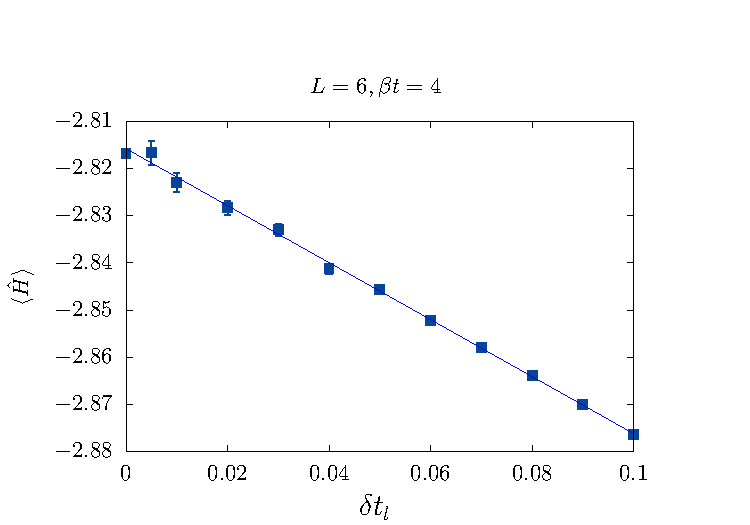
\includegraphics[scale=0.9,clip]{Figures/Langevin.pdf}
            \end{center}
        \caption{Total energy for the 6-site Hubbard chain at $U/t=4$, $\beta t = 4$ and with open boundary conditions. For this system it can be shown that the determinant is always positive, so that no singularities occur in the action and, consequently, the Langevin dynamics works very well.  The reference data point at $\delta \tl =0$ comes from the discrete field code for the field coupled to the z-component of the magnetization and reads $-2.8169 \pm 0.0013$, while the extrapolated value is $-2.8176 \pm 0.0010$. Throughout the runs the maximal force remained bellow the threshold of 1.5. The displayed data has been produced by the pyALF script 
         \href{https://git.physik.uni-wuerzburg.de/ALF/pyALF/-/blob/master/Scripts/Langevin.py}{\texttt{Langevin.py}}. }\label{Langevin.fig}
\end{figure}

